% TODO: Punkte pro Aufgabe vergeben
% TODO: Titelblatt re Word
\documentclass[10pt,ngerman]{examdesign}
\usepackage[utf8]{inputenc}
\usepackage[T1]{fontenc}
\usepackage{listings}
\usepackage{graphicx}

\Fullpages
\NumberOfVersions{1}
\SectionPrefix{Abschnitt \arabic{sectionindex}. \space}
\lstset{language=Java,numbers=left}
\IncludeFromFile{listings.tex}
\ContinuousNumbering

\begin{document}

\begin{examtop}
    %\parbox{8cm}{
    %    1. Leistungs\"uberpr\"ufung Fr\"uhlingssemester 2012\\
    %    Webprogrammieren I\\
    %    Lafon \\
    %    Dauer der Pr\"ufung: 60min \\
    %    Erlaubte Hilfsmittel:\\
    %      Folien, Mitschriebe aus der Vorlesung\\
    %    }
    \hfill
    \parbox{10cm}{
    Name: \hrulefill\\[5pt]
    Klasse: \hrulefill\\[5pt]
    Datum: \hrulefill}
    \bigskip

  %\begin{itemize}
  %   \item Markieren Sie richtige Antworten mit einem Kreuz.
  %   \item Falls Sie sich umentscheiden sollten und eine bereits als richtig
  %   markierte Antwort trotzdem als nicht richtig bezeichnen m\"ochten, machen Sie
  %   einen Kreis um das Kreuz.
  %   \item Pro Frage k\"onnen keine, eine oder mehrere Antworten richtig sein.
  %   \item Antworten welche als richtig markiert wurden, jedoch falsch sind, geben
  %   einen Punkt Abzug.
  %   \item Falls Ihnen eine Frage nicht klar sein sollte, treffen Sie eine Annahme
  %   und halten Sie diese schriftlich fest.
  %   \item F\"ur jede Aufgabe ist ein separates Blatt zu verwenden.
  %   \item Die L\"osungsbl\"atter sind nur einseitig zu beschriften
  %   \item Sämtliche Arbeiten sind absolut selbständig auszuführen. Wer sich unredlich verhält,
  %  wird unmittelbar nach Feststellung des Tatbestandes von der Prüfung ausgeschlossen.
  %  In diesem Fall  gilt die ganze Prüfung als nicht bestanden.  Bei  besonders
  %  schwerwiegender Unredlichkeit wird der fehlbare Studierende aus der Schule
  %  ausgeschlossen.
  %\end{itemize}

\end{examtop}
\pagebreak

\begin{multiplechoice}

  \begin{question}
    (1pt) - Welche Eigenschaften bringt man mit DNS in Verbindung?
    \choice[!]{"Hierarchisch"}
    \choice[!]{"Redundant"}
    \choice[!]{"Dezentral"}
    \choice[]{"Flach"}
    \smallskip
  \end{question}

  \begin{question}
    (1pt) - Wie heisst die Transportschicht im Browser?
    \choice[]{"SOAP"}
    \choice[!]{"HTTP"}
    \choice[]{"WebDAV"}
    \choice[]{"REST"}
    \smallskip
  \end{question}

  \begin{question}
    (1pt) - Was sind die gängigen Port(s) für HTTP(S)?
    \choice[!]{"80"}
    \choice[]{"21"}
    \choice[]{"23"}
    \smallskip
  \end{question}

  \begin{question}
    (1pt) - Welche Tags sind semantisch?
    \choice[!]{"q"}
    \choice[]{"div"}
    \choice[!]{"a"}
    \smallskip
  \end{question}

  \begin{question}
    (1pt) - Wof\"ur steht URI?
    \choice[]{"Unique Resource Indicator"}
    \choice[]{"Uniform Resource Locator"}
    \choice[!]{"Uniform Resource Identifier"}
    \choice[!]{"Das ist in Kanton in der Schweiz"}
    \smallskip
  \end{question}

\end{multiplechoice}


\begin{shortanswer}

  \begin{question}
    (4pt) - Skizzieren Sie wie der Browser folgenden Quellcode rendert!
    \InsertChunk{skizzehtml}{html}
    \InsertChunk{skizzecss}{css}
    \begin{answer}
      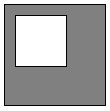
\includegraphics{margins.jpg}
    \end{answer}
  \end{question}

  \begin{question}
    (1pt) - Worin unterscheidet sich das Verhalten von 'margin' bei inline und block
    Elementen?
    \begin{answer}
    inline: margins werden addiert,
    block: margins werden kollabiert
    \end{answer}
  \end{question}

  \begin{question}
    (10pt) - Summieren Sie alle geraden Werte der Fibonacci Sequenz von 1 bis 4'000'000
     in Javasript. Wenn m\"oglich, achten Sie auf eine effiziente
     Implementierung. Zur Erinnerung; die Fibonacci Sequenz ist wie folgt
    definiert:\\
    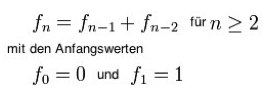
\includegraphics[width=60mm]{fibonacci.jpg}
    \begin{answer}
      \InsertChunk{answerFib1}{Analog zur bereits gezeigten Loesung}
      \InsertChunk{answerFib2}
    \end{answer}
  \end{question}

  \begin{question}
    (2pt) - Nennen Sie stichwortartig Vorteile der besseren Code Beispiels!
    \InsertChunk{semantichtml}{code sample 1}
    \InsertChunk{nonsemantichtml}{code sample 2}
    \begin{answer}
      Durch Semantik:
      \begin{itemize}
        \item Besser lesbarer Code
        \item SEO Optimierung
        \item Accessibility
        \item Code Styling auf semantischer Ebene ohne Klassen/IDs
      \end{itemize}
    \end{answer}
  \end{question}

  %\begin{question}
  %  Notieren Sie die Syntax von URL!
  %  \begin{answer}
  %    \InsertChunk{answerURL}
  %  \end{answer}
  %\end{question}

  \begin{question}
    (2pt) - Ihr Kunde m\"ochte eine Webseite haben mit einem animierten
    Baustellenschild dessen Tooltip lautet: "Hier ensteht eine neue
    Internetpr\"asenz!". Beim Click auf das Baustellenschild soll sich ein
    neues Browserfenster mit der alten Webseite des Kunden(c2.com) \"offnen.
    Schreiben Sie den dazu notwendigen Inhalt des HTML <body>!
    \begin{answer}
      \InsertChunk{answerBaustelle}
    \end{answer}
  \end{question}

  \begin{question}
    (1pt) - Wozu dient 'charset' im 'content' Attribut des 'meta' Tags?
    \begin{answer}
      Gibt die Zeichenkodierung im Dokument an.
    \end{answer}
  \end{question}

  \begin{block}
    \begin{question}
      (1pt) - Was haben die folgenden Farben gemein?
      \InsertChunk{greyish}
      \begin{answer}
        Alles Graut\"one
      \end{answer}
    \end{question}

    \begin{question}
      (1pt) - Was haben die folgenden Farben gemein?
      \InsertChunk{redish}
      \begin{answer}
        Alles r\"otliche Farben
      \end{answer}
    \end{question}
  \end{block}

  \begin{question}
    (1pt) - Wann setzt man CSS Pseudo Klassen ein?
    \begin{answer}
      \begin{itemize}
        \item Verschiedene Zust\"ande eines Elementes
        \item Algorithmische Selektoren(ehemals Javascript)
      \end{itemize}
    \end{answer}
  \end{question}

\end{shortanswer}

\begin{truefalse}
  15. (1pt) - Welche Tags sind inline(i), welche block(b) Elemente?
  \begin{question}
    \answer{b} div
  \end{question}
  \begin{question}
    \answer{i} span
  \end{question}
  \begin{question}
    \answer{i} q
  \end{question}
  \begin{question}
    \answer{b} p
  \end{question}
  \begin{question}
    \answer{i} a
  \end{question}
\end{truefalse}


%\begin{truefalse}
%  Bringen Sie die folgenden Technologien in die Reihenfolge der jeweiligen
%  Entstehung!
%  \begin{question}
%    \answer{1} SGML
%  \end{question}
%  \begin{question}
%    \answer{4} HTML5
%  \end{question}
%  \begin{question}
%    \answer{3} XHTML1
%  \end{question}
%  \begin{question}
%    \answer{2} HTML4
%  \end{question}
%\end{truefalse}

\begin{truefalse}
  16. (2pt) - Bringen Sie die Begriffe 'padding', 'content', 'margin', 'border'  in Bezug
  auf das CSS Box Modell in die richtige Reihenfolge!
  \begin{question}
    \answer{1} content
  \end{question}
  \begin{question}
    \answer{2} padding
  \end{question}
  \begin{question}
    \answer{3} border
  \end{question}
  \begin{question}
    \answer{4} margin
  \end{question}
\end{truefalse}

\begin{truefalse}
  17. (2pt) - Welche Aussagen treffen auf die Positionierung 'static'(s), 'absolute'(a), 'relative'(r), 'fixed'(f) zu?
  \begin{question}
    \answer{absolute} Elemente sind relativ zum ersten \"Ubergeordneten Element positioniert, welches nicht 'static' ist
  \end{question}
  \begin{question}
    \answer{fixed} Elemente bewegen sich nicht, selbst wenn das Fenster scrollt
  \end{question}
  \begin{question}
    \answer{relative} Elemente sind verh\"altnissm\"assig zu ihrer normalen Position positioniert
  \end{question}
  \begin{question}
    \answer{static} Elemente bewegen sich immer relativ zum normalen Fluss der Seite
  \end{question}
\end{truefalse}

  \begin{truefalse}
    18. (2pt) - In welcher Farbe werden die folgenden Textbl\"ocke im Browser angezeigt?
    \InsertChunk{cascadecss}{css}
    \InsertChunk{cascadehtml}{html}
    \begin{question}
      \answer{green} punished
    \end{question}
    \begin{question}
      \answer{green} will
    \end{question}
    \begin{question}
      \answer{blue} anger
    \end{question}
    \begin{question}
      \answer{blue} Restlicher Text
    \end{question}
  \end{truefalse}

%\begin{shortanswer}
%  \begin{question}
%    \"Andern Sie den Quellcode von A20 so, dass 'Buddha' rot dargestellt wird.
%    \begin{answer}
%      \InsertChunk{redhtml}
%      \InsertChunk{redcss}
%    \end{answer}
%  \end{question}
%\end{shortanswer}

\end{document}

